\title{Lab Assignment 2 \\ \small{Datamining}}
\author{Chiel ten Brinke 3677133}
\documentclass[12pt]{article}
\usepackage{amssymb,amsmath,amsthm,enumerate,graphicx,float,lmodern,xparse}

\newtheorem{theorem}{Theorem}[section]
\newtheorem{lemma}[theorem]{Lemma}
\newtheorem{proposition}[theorem]{Proposition}
\newtheorem{corollary}[theorem]{Corollary}

\theoremstyle{definition}
\newtheorem{definition}[theorem]{Definition}
\newtheorem{axiom}[theorem]{Axiom}
\newtheorem{example}[theorem]{Example}
\newtheorem{remark}[theorem]{Remark}

%\newcommand{\set}[1]{\left\lbrace#1\right\rbrace}
%\newcommand{\set}[2]{\left\lbrace#1 \, \middle|\, #2 \right\rbrace}
\NewDocumentCommand\set{mg}{%
    \ensuremath{\left\lbrace #1 \IfNoValueTF{#2}{}{\, \middle|\, #2} \right\rbrace}%
}

\begin{document}
\maketitle

\section*{Notes}
\begin{itemize}
    \item The Bron-Kerbosch algorithm has not been taken from the site, but has been implemented manually.
    \item For all computations we used the same seed, namely 37.
\end{itemize}

\section*{a}
There are 10 variables, so there are $\frac{10 \cdot 9}{2} = 45$ undirected edges.
Since each combination of edges represents exactly one graphical model,
there are $2^{45} = 35184372088832$ possible graphical models.

\section*{b}
The table of counts has a cell for each combination of variable values.
This comes down to $9 \cdot 2 \cdot 2 \cdot 2 \cdot 3 \cdot 6 \cdot 4 \cdot 3 \cdot 5 \cdot 2 = 155520$ possible combinations.
This is confirmed by taking the length function of the table of counts in R.
The number of parameters of the saturated model equals the number of cells in the table of counts.

\section*{c}
\paragraph{Cliques}
$\set{1,3,10}$, $\set{1,8}$, $\set{1,9}$, $\set{2,8}$, $\set{2,9}$, $\set{2,10}$, $\set{3,6}$,
$\set{4,6}$, $\set{5,6}$, $\set{5,10}$, $\set{6,7}$, $\set{6,8}$, $\set{6, 9}$

\paragraph{BIC Score} 15841.66

\paragraph{Graph} See Figure~\ref{fig:c}

\begin{figure}[H]
    \centering
    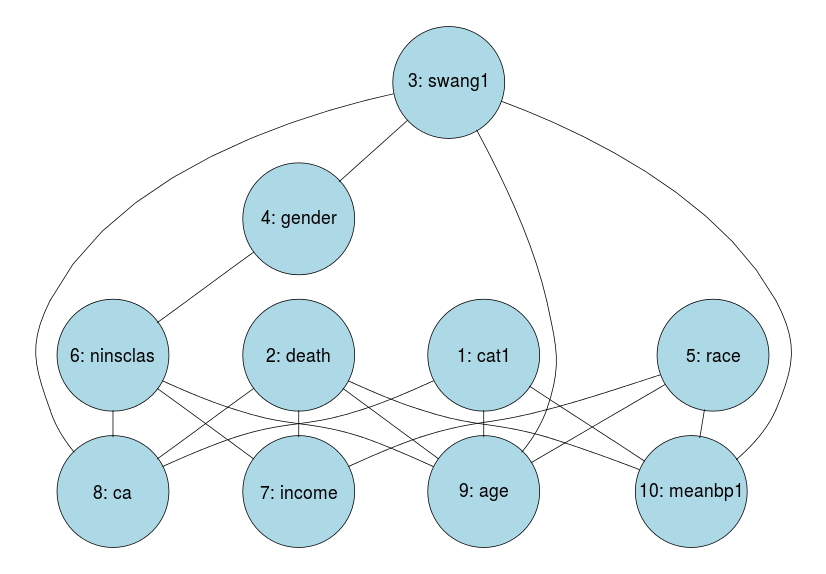
\includegraphics[width=0.8\linewidth]{c.png}
    \caption{Independence graph of backward forward search from empty graph using BIC.}
\label{fig:c}
\end{figure}

\section*{d}
Income and gender are independent given ninsclas, because of the separator property.
To predict whether a patient will survive, we only need ca, age and meanbp1, because
death is independent of all other variables when these are given.

\section*{e}
\paragraph{Cliques}
$\set{1,3,10}$, $\set{1,8}$, $\set{2,7}$, $\set{2,8}$, $\set{2,9}$, $\set{2,10}$,
$\set{3,4}$, $\set{3,9}$, $\set{4,6}$, $\set{5,7}$, $\set{5,9}$, $\set{5,10}$,
$\set{6,7}$, $\set{6,8}$, $\set{6,9}$

\paragraph{BIC Score} 15850.53

\paragraph{Graph} See Figure~\ref{fig:e}

\begin{figure}[H]
    \centering
    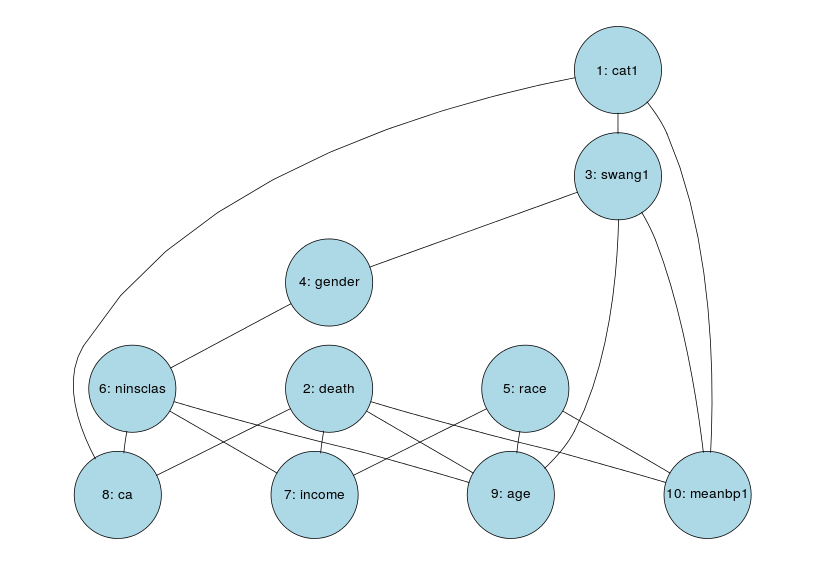
\includegraphics[width=0.8\linewidth]{e.png}
    \caption{Independence graph of backward forward search from complete graph using BIC.}
\label{fig:e}
\end{figure}

This model has a lower (thus better) BIC score than the model generated in c.
So this model is considered to be a better model.

\section*{f}
In both cases the algorithm gives the same result.

\paragraph{Cliques}
$\set{1,2,8}$, $\set{1,2,9}$, $\set{1,2,10}$, $\set{1,3,9}$, $\set{1,3,10}$, $\set{1,4,8}$,
$\set{1,4,10}$, $\set{3,6,9}$, $\set{4,5,6}$, $\set{4,5,10}$, $\set{4,8,6}$, $\set{7,2}$,
$\set{7,5,6}$, $\set{9,5,6}$

\paragraph{AIC Score} 14278.21

\paragraph{Graph} See Figure~\ref{fig:f}

\begin{figure}[H]
    \centering
    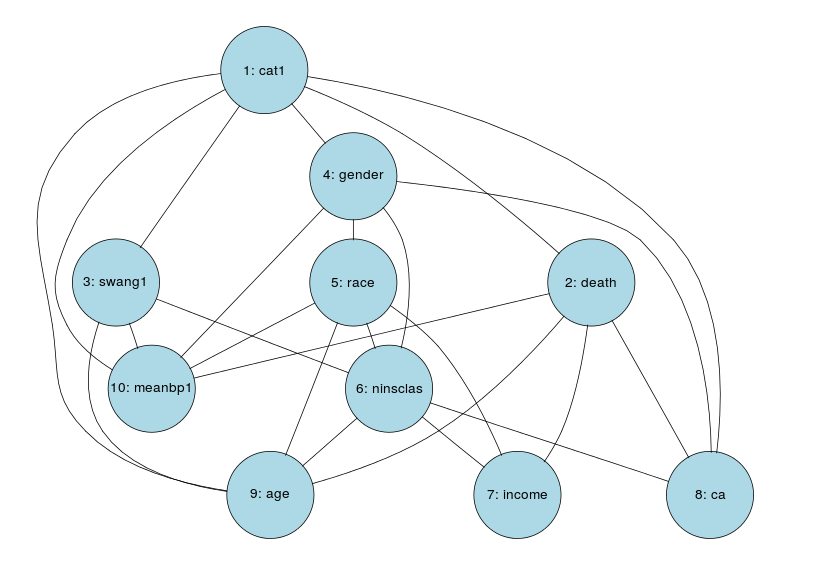
\includegraphics[width=0.8\linewidth]{f.png}
    \caption{Independence graph of backward forward search from empty graph or complete graph using AIC.}
\label{fig:f}
\end{figure}

%\subsection*{From complete graph}
%\paragraph{Cliques}
%$\set{1,2,8}$, $\set{1,2,10}$, $\set{1,4,3}$, $\set{1,4,8}$, $\set{1,6}$, $\set{1,10,3}$,
%$\set{7,2}$, $\set{7,3,4}$, $\set{7,5,6}$, $\set{8,2,9}$, $\set{8,4,9}$, $\set{9,3,4}$,
%$\set{9,5,6}$, $\set{10,5}$

%\paragraph{AIC Score} 14278.21

%\paragraph{Graph} See Figure~\ref{fig:f2}

%\begin{figure}[H]
    %\centering
    %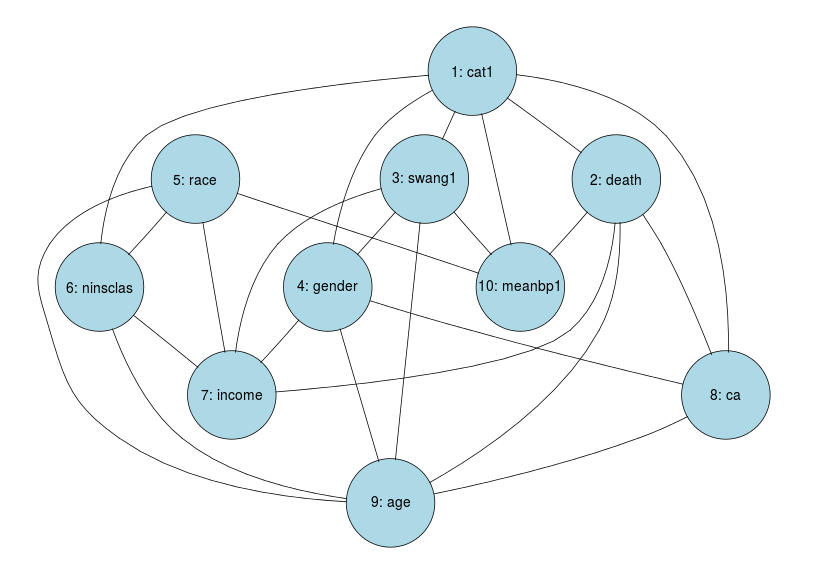
\includegraphics[width=0.8\linewidth]{f2.png}
    %\caption{Independence graph of backward forward search from complete graph using AIC.}
%\label{fig:f2}
%\end{figure}

%The two resulting models are almost the same, but there are some small differences.

\section*{g}
The models found with AIC are more complex than the models found with BIC.
This is because BIC penalizes complex models harder than AIC.

\section*{h}
To get a first impression of how the parameters nstart and prob relate to the score functions,
let us perform series of small tests for varying parameters and construct a 3d graph from this.
To keep the compution time within reasonable bounds, we work with a randomly sampled subset
from the original dataset.
Moreover, we will not consider all 10 variables during the hill climbing part, but only a subset.
For each configuraton of the parameters, we run the hill climbing algorithm 10 times with 4
randomly chosen variables.
The average score of these runs is taken to be the final outcome for this configuraton.
This will not give a completely reliable result, but hopefully it will give an approximate
idea of how the parameters nstart and prob influence the quality of the model.
The result is shown in Figure~\ref{fig:rough}.

\begin{figure}[H]
    \centering
    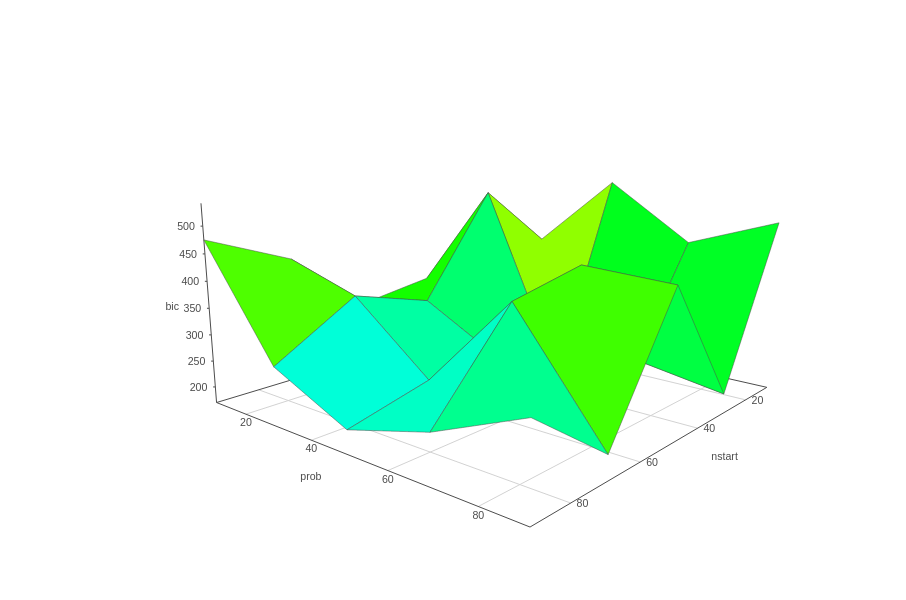
\includegraphics[width=0.8\linewidth]{rough2.png}
    \caption{BIC score as a function of nstart and prob.}
\label{fig:rough}
\end{figure}

As one can see, the graph is not entirely unambiguous but the best scores seem to
center around the point where prob is around 0.5 and nstart is as high as possible.
The latter is very natural, as the result cannot get worse when more restarts are done.

Keeping this in mind, we perform several runs on the full dataset and using all variables.
The results are stated in Table~\ref{table1}.

\begin{table}[H]
\centering
\begin{tabular}{llll}
    nstart & prob & AIC & BIC \\
    \hline \hline
    1 & 0.4 & 14344.95 & 15791.47 \\
    1 & 0.5 & 14341.64 & 15905.87 \\
    1 & 0.6 & 14341.64 & 15791.47 \\
    5 & 0.4 & 14263.97 & 15783.74 \\
    5 & 0.5 & 14278.21 & 15849.38 \\
    5 & 0.6 & 14263.97 & 15783.74 \\
    10 & 0.4 & 14263.97 & 15783.74 \\
    10 & 0.5 & 14263.97 & 15783.74 \\
    10 & 0.6 & 14263.97 & 15783.74 \\
\end{tabular}
\caption{AIC score as a function of nstart and prob.}
\label{table1}
\end{table}

Thus the model with the best BIC score is the following.
\paragraph{Cliques}
$\set{1,3,10}$, $\set{1,8}$, $\set{1,9}$, $\set{2,7}$, $\set{2,8}$, $\set{2,9}$,
$\set{2,10}$, $\set{4,6}$, $\set{5,7}$, $\set{5,9}$, $\set{5,10}$, $\set{6,3}$,
$\set{6,7}$, $\set{6,8}$, $\set{6,9}$

\paragraph{BIC Score} 15783.74

\paragraph{Graph} See Figure~\ref{fig:best}

\begin{figure}[H]
    \centering
    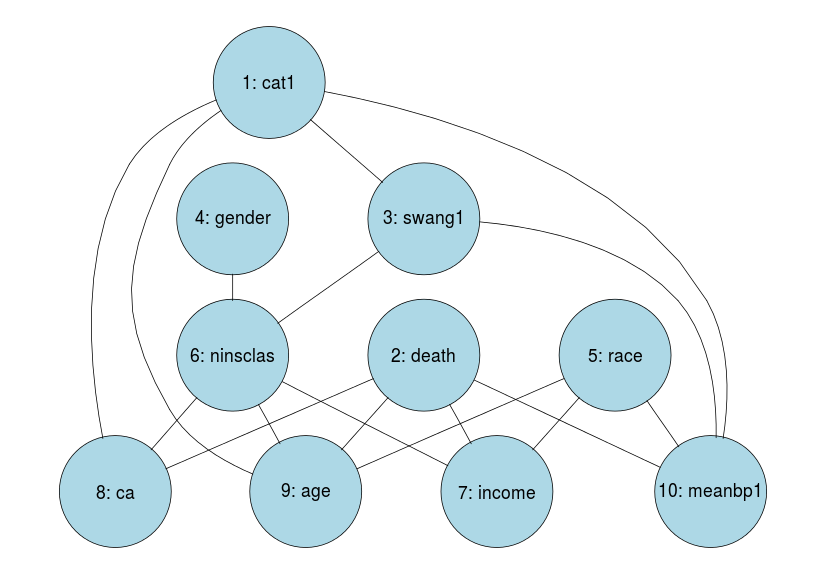
\includegraphics[width=0.8\linewidth]{best.png}
    \caption{Independence graph of model with best BIC score.}
\label{fig:best}
\end{figure}

\end{document}
